\documentclass[10pt, landscape]{article}
\usepackage[scaled=0.92]{helvet}
\usepackage{calc}
\usepackage{multicol}
\usepackage{ifthen}
\usepackage[a4paper,margin=5mm,landscape]{geometry}
\usepackage{amsmath,amsthm,amsfonts,amssymb}
\usepackage{color,graphicx,overpic}
\usepackage{hyperref}
\usepackage{newtxtext} 
\usepackage{enumitem}
\usepackage{amssymb}
\usepackage[table]{xcolor}
\usepackage{vwcol}
\usepackage{tikz}
\usetikzlibrary{arrows.meta}
\usetikzlibrary{calc}
\usepackage{mathtools}
\usepackage{nicematrix}
\usepackage[T1]{fontenc} %%% <--- NOTE THIS
% for relations
\usepackage{cancel}
\usepackage{ mathrsfs }
\usepackage{listings}
\usepackage{background}
\setlist{nosep}

\usepackage{etoolbox}
\makeatletter
\preto{\@verbatim}{\topsep=0pt \partopsep=0pt }
\makeatother

\backgroundsetup{
scale=1,
color=black,
opacity=0.4,
angle=0,
contents={%
  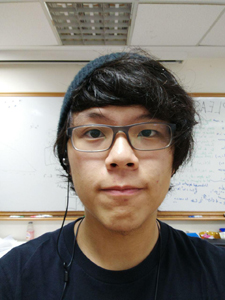
\includegraphics[width=\paperwidth,height=\paperheight]{eldon.png}
  }%
}

\pdfinfo{
  /Title (CS2040S.pdf)
  /Creator (TeX)
  /Producer (pdfTeX 1.40.0)
  /Author (Seamus)
  /Subject (Example)
  /Keywords (pdflatex, latex,pdftex,tex)}

\lstset{language=Java,keywordstyle={\bfseries \color{black}}}

% Turn off header and footer
\pagestyle{empty}

\newenvironment{tightcenter}{%
  \setlength\topsep{0pt}
  \setlength\parskip{0pt}
  \begin{center}
}{%
  \end{center}
}

% redefine section commands to use less space
\makeatletter
\renewcommand{\section}{\@startsection{section}{1}{0mm}%
                                {-1ex plus -.5ex minus -.2ex}%
                                {0.5ex plus .2ex}%x
                                {\normalfont\large\bfseries}}
\renewcommand{\section}{\@startsection{section}{2}{0mm}%
                                {-1explus -.5ex minus -.2ex}%
                                {0.5ex plus .2ex}%
                                {\normalfont\normalsize\bfseries}}
\renewcommand{\subsection}{\@startsection{subsection}{3}{0mm}%
                                {-1ex plus -.5ex minus -.2ex}%
                                {1ex plus .2ex}%
                                {\normalfont\small\bfseries}}%
\renewcommand{\familydefault}{\sfdefault}
\renewcommand\rmdefault{\sfdefault}
% makes nested numbering (e.g. 1.1.1, 1.1.2, etc)
\renewcommand{\labelenumii}{\theenumii}
\renewcommand{\theenumii}{\theenumi.\arabic{enumii}.}
\renewcommand\labelitemii{•}
%  for logical not operator
\renewcommand{\lnot}{\mathord{\sim}}
\renewcommand{\bf}[1]{\textbf{#1}}
\newcommand{\abs}[1]{\vert #1 \vert}
\newcommand{\Mod}[1]{\ \mathrm{mod}\ #1}

\makeatother
\definecolor{myblue}{cmyk}{1,.72,0,.38}
\everymath\expandafter{\the\everymath \color{myblue}}
% Define BibTeX command
\def\BibTeX{{\rm B\kern-.05em{\sc i\kern-.025em b}\kern-.08em
    T\kern-.1667em\lower.7ex\hbox{E}\kern-.125emX}}
\let\iff\leftrightarrow
\let\Iff\Leftrightarrow
\let\then\rightarrow
\let\Then\Rightarrow

% Don't print section numbers
\setcounter{secnumdepth}{0}

\setlength{\parindent}{0pt}
\setlength{\parskip}{0pt plus 0.5ex}
%% this changes all items (enumerate and itemize)
\setlength{\leftmargini}{0.5cm}
\setlength{\leftmarginii}{0.5cm}
\setlist[itemize,1]{leftmargin=2mm,labelindent=1mm,labelsep=1mm}
\setlist[itemize,2]{leftmargin=4mm,labelindent=1mm,labelsep=1mm}

%My Environments
\newtheorem{example}[section]{Example}
% -----------------------------------------------------------------------

\begin{document}
\raggedright
\footnotesize
\begin{multicols*}{4}

% multicol parameters
% These lengths are set only within the two main columns
\setlength{\columnseprule}{0.25pt}
\setlength{\premulticols}{1pt}
\setlength{\postmulticols}{1pt}
\setlength{\multicolsep}{1pt}
\setlength{\columnsep}{2pt}

\begin{center}
    \fbox{%
        \parbox{0.8\linewidth}{\centering \textcolor{black}{
            {\Large\textbf{CS2040S}}
            \\ \normalsize{AY24/25 Sem 2}}
            \\ {\footnotesize \textcolor{myblue}{by ngmh}} 
        }%
    }
\end{center}

\section{Big-O}
\begin{itemize}
    \item $T(n)=$ running time on input with size $n$
    \item Upper Bound: $T(n)=O(f(n))$ if $T$ grows no faster than $f$, i.e. $\exists\ c > 0, n_0 > 0$ such that $\forall \ n > n_0, T(n) \leq cf(n)$
    \item Lower Bound: $T(n)=\Omega(f(n))$ if $T$ grows no slower than $f$, i.e. $\exists\ c > 0, n_0 > 0$ such that $\forall \ n > n_0, T(n) \geq cf(n)$
    \item Tight Bound: $T(n)=\Theta(f(n))$ if and only if $T(n)=O(f(n))=\Omega(f(n))$
    \item $log(n!)=\Theta(n\ log\ n)$ considering $log(n/2)$ and $log(n)$
    \item String append is $O(n)$ in Java
    \item Master Theorem: For $T(n)=aT(n/b)+cn^k$, $T(1)=c$, compare $a$ and $b^k$, $<: \Theta(n^k)$, $=:\Theta(n^k \ log \ n)$, $>: \Theta(n^{log_ba})$
    \item $T(n)=2T(n/2)+O(n\ log \ n)=O(n\ log^2\ n)$, $T(n)=2T(n/4)+O(1)=O(\sqrt{n})$
    \item Fibonacci: $O(\phi^n)$, proof by induction, $T(n)=T(n-1)+T(n-2)+O(1)$, $T(i)=F(i)-1$
    \item $log(n)<\sqrt{n}$, $log^k(n)<n^m$, $n^{log(n)}<2^n$
\end{itemize}

\section{Binary Search}
\begin{itemize}
    \item Precondition: True when function begins, important for it to work correctly, e.g. array has size $n$ and is sorted
    \item Postcondition: True when function ends, useful to show computation was done correctly, e.g. if element is in array, $A[begin]=key$
    \item Invariant: Relationship between variables which is always true, e.g. $A[begin] \leq key \leq A[end]$ and $end-begin \leq n/2^k$ for iteration $k$
\end{itemize}
\begin{verbatim}
    int search(A, key, n)
        begin = 0; end = n-1
        while begin < end do:
            mid = begin + (end-begin)/2
            if key <= A[mid]: end = mid
            else: begin = mid+1
        return (A[begin]==key) ? begin : -1
\end{verbatim}

\section{Peak Finding}
\begin{itemize}
    \item Find local maximum $A[i-1] \leq A[i] \geq A[i+1]$
    \item Invariant: There exists a peak in $[begin, end]$ which is also a peak in $[0, n-1]$
\end{itemize}
\begin{verbatim}
    FindPeak(A, n)
        if A[n/2] is a peak then return n/2
        else if A[n/2+1] > A[n/2] then
            Search for peak in right half
        else if A[n/2-1] > A[n/2] then
            Search for peak in left half
\end{verbatim}
\begin{itemize}
    \item Steep Peak: $A[i-1] < A[i] > A[i+1]$
    \item Fails on case where both sides are equal, degenerates to $O(n)$ when recursing on both halves
    \item Slow 2D Peak Finding: Find global max in each columnn, find peak in array of maximums, $O(mn+log(m))$
    \item Fast 2D Peak Finding: Find peak in array of peaks with lazy evaluation of columns, recurse on half by comparing max of adjacent columns, $O(n\ log\ m)$
\end{itemize}

\section{Sorting}
\subsection{Bubble Sort}
\begin{itemize}
    \item Loop through array $n$ times, swapping adjacent elements that are out of order
    \item Best Case: Sorted, $O(n)$, Average / Worst Case: $O(n^2)$
    \item Invariant: After iteration $j$, the biggest $j$ items are sorted in the last $j$ positions of the array
\end{itemize}
\subsection{Selection Sort}
\begin{itemize}
    \item Repeatedly find minimum element and add to sorted prefix
    \item Always $O(n^2)$
    \item Invariant: After iteration $j$, the smallest $j$ items are sorted in the first $j$ positions of the array
\end{itemize}
\subsection{Insertion Sort}
\begin{itemize}
    \item Loop from front, bubbling current element downwards into correct place in prefix
    \item Best Case: Sorted, $O(n)$, Average / Worst Case: $O(n^2)$
    \item Invariant: After iteration $j$, the first $j$ items in the array are sorted
\end{itemize}
\subsection{Merge Sort}
\begin{itemize}
    \item Divide and conquer, sort both halves of array, then merge back together
    \item $T(n)=2T(n/2)+cn=O(n \ log \ n)$
    \item $log \ n$ levels, each with $n$ elements total
\end{itemize}
\subsection{Quick Sort}
\begin{itemize}
    \item Unlike mergesort, partition array by a pivot before recursing
    \item Average Case: $O(n \ log \ n)$, Worst Case: $O(n^2)$
    \item Not In-Place Partition: Create new array, if current element is lower than pivot add to prefix, else add to suffix using two pointers
    \item In-Place Partition: Move low pointer until it is larger than pivot, move high pointer until it is not larger than pivot, then swap until both pointer cross
    \item Invariants: $A[high]> pivot$ after each loop, and for all $i \geq high, A[i] > pivot$ and for all $1 < j < low, A[j] < pivot$
\end{itemize}
    \begin{verbatim}
swap(A[1], A[pIndex])
while (low < high)
    while (A[low] <= p) and (low < high) low++
    while (A[high] > p) and (low < high) high--
    if (low < high) swap(A[low], A[high])
swap(A[l], A[low-1])
    \end{verbatim}
\begin{itemize}
    \item Two Pass 3-Way Partition: Regular partition, packing with duplicates after
    \item One Pass 3-Way Partition: Maintain four regions of array ($<pivot, =pivot, in \ progress, > pivot$)
    \item Compare $A[i]$ and $pivot$, $<$: swap with start of $=pivot$, $==$: increment $=pivot$ end, $>$: swap with start of $> pivot$
\end{itemize}
\subsection{Paranoid QuickSort}
\begin{itemize}
    \item Partition until certain factor is met, e.g. $9/10$
    \item Probability of good pivot is $8/10$, so $E[Partitions]=1/p=10/8<2$, so by expectation we only have to partition twice
    \item $E[T(n)]=E[T(k)]+E[T(n-k)]+E[Partitions](n) \leq E[T(k)]+E[T(n-k)]+2n=O(n \ log \ n)$
    \item $T(n)=T(n/10)+T(9n/10)+O(n)=O(n \ log \ n)$
\end{itemize}

\subsection{Properties}
\begin{itemize}
    \item MergeSort and QuickSort are not in-place
    \item Stability: Preserving initial order of equal elements
    \item SelectionSort and QuickSort are not stable due to swaps
    \item Swap first and last element to differentiate between Insertion and Bubble Complexity
\end{itemize}

\subsection{Quick Select}
\begin{itemize}
    \item Select $k^{th}$ smallest element in unsorted array
    \item Randomly partition (with paranoia if wanted), recursing only on the correct half, $O(n)$ expected
    \item $E[T(n)]\leq E[T(9n/10)]+E[Partitions](n) \leq E[T(9n/10)]+2n \leq O(n)$
\end{itemize}

\section{Trees}
\begin{itemize}
    \item Binary Search Tree: $left \ keys < key < right \ keys$
    \item Height: $0$ at leaf, increases by $1$ for each parent after taking maximum of children
    \item Minimum / Maximum: Keep traversing left / right until leaf
    \item Search / Insertion: Keep recursing on correct child until leaf, inserting if needed
    \item In-Order: LSR, Pre-Order: SLR, Post-Order: LRS, Level-Order: Increasing distance from root, left to right
    \item Successor: Search for key, if $result > key$, return $result$, else return $successor(result)$
    \item $successor(key):$ If right tree exists, take its min. If not, recurse upwards until we are in a left subtree, then return parent (so that $parent > key$
    \item 1-Child Deletion: Remove $v$, connect $child(v)$ to $parent(v)$
    \item 2-Child Deletion: Let $x = successor(v)$. Replace $v$ with $x$, then replace $x$ with its right child, works as $x$ cannot have a left child
    \item Order Statistics: Rank and Select, use subtree size information to determine where to recurse, like quick select
    \item Rank is $left.w+1$, if selecting right $right.select(k-rank)$, if node is right child repeatedly add $par.left.w+1$
    \item Counting Inversions: For each element, use order statistics to get inversion count of it as $tree\ size - rank(element)$
    \item $(a,b)-$tree: $2\leq a\leq (b+1)/2$, $O(log \ n)$ operations, $[a, b]$ number of children
    \item Virus Problem: Find minimum possible number of days for every node to be visited, each day a node can visit any adjacent node, binary search and partition by each edge along path between 2 sources, solve single source case
    \item Tries: Store multiple strings in a tree, with letters as nodes, words are paths from root to leaf, use special mark for terminal character
\end{itemize}

\section{AVL Trees}
\begin{itemize}
    \item Balanced: $h=O(log \ n)$
    \item Perfectly Balanced: For any node both subtrees have same height
    \item Height Balanced: $|v.left.h-v.right.h|\leq 1$, has at most $h<2log(n)$, and $n>2^{h/2}$
    \item Weight Balanced: $v.left.w, v.right.w \leq \alpha \cdot v.w$
    \item Scapegoat Tree: $2/3$ weight balanced, rebuild tree at highest unbalanced node if necessary
    \item Maximally Imbalanced: Tree with minimum possible nodes given a total height, construct recursively
    \item Left / Right Heavy: Child with greater height
    \item Rotations: Direction is where root of subtree goes, requires child opposite of rotation direction
    \item If middle heavy, rotate child away from middle before rotating root
    \begin{itemize}
        \item v Left
        Heavy: Check Left child:
        \begin{itemize}
            \item Balanced: Right-Rotate(v)
            \item Left Heavy: Right-Rotate(v)
            \item Right Heavy: Left-Rotate(v.left), Right-Rotate(v)
        \end{itemize}
        \item v Right
        Heavy, Check Right child:
        \begin{itemize}
            \item Balanced: Left-Rotate(v)
            \item Left Heavy: Right-Rotate(v.right), Left-Rotate(v)
            \item Right Heavy: Left-Rotate(v)
        \end{itemize}
    \end{itemize}
    \item Insertion: Only need to fix lowest unbalanced node with at most two rotations, since insertion increases height and rotation reduces height
    \item Deletion: After deletion, for every ancestor of deleted node, rotate if not height-balanced, $O(log \ n)$, as rotation and deletion both reduce height
    \item Modification: Only store difference in height from parent
\end{itemize}

\section{Hashing}
\begin{itemize}
    \item Direct Access Table: Table indexed by keys, but faces size problem
    \item Hash Function: Map large set of possible keys to smaller set of actual keys / buckets
    \item Collision: Two distinct keys map to same bucket
    \item Chaining: Each bucket is a linked list, insertion appends to front
    \item Insertion is $O(1)$, Search is worst case $O(n)$
    \item Simple Uniform Hashing Assumption: Each key is equally likely to map to every bucket and is mapped independently
    \item $load(table)=n/m$ where $n$ is items and $m$ is buckets, expected search time is $O(1)+n/m$, when $m=\Omega(n)$ e.g. $m=2n$, expected search time is $O(1)$
    \item Expected maximum cost of inserting $n$ elements is $O(log\ n)$ or $\Theta(log \ n/log\ log\ n)$
    \item In Java, keys should be immutable, and implement $int\ hashCode()$
    \item Must return same value if object hasn't changed, and two equal objects must return the same hashCode, uses $hash()$ to ensure that similar hashCodes have a bounded number of collisions
    \item Open Addressing: Insert items into table directly
    \item If hash position is occupied, increment and continue probing, need not be linear
    \item Tombstoning: Use marker for deleted elements, to indicate for probing to continue, replace on insertion, if too many tombstones, rehash the table
    \item Insertion Resizing: Double table size when full, total cost is $O(n)$ for resizing with $O(1)$ insertion on average
    \item Deletion Resizing: Halve table size when quarter full
    \item Amortised Analysis: Inserting $n$ elements, most will have cost $O(1)$, some have cost $O(k)$, in total will be $O(n)$ for $n$ operations, so amortised is $O(1)$, can extend idea to deletion and resizing as well
    \item Linear probing results in clusters, if quarter full has clusters of size $\Omega(log \ n)$, but is still faster in practice
    \item Merkle Tree: Each node is the hash of the concatenation of the child nodes
    \item Cuckoo Hashing: Two hash tables with own keys, kick existing key to other table on collision, but fails if infinite loop, $O(1)$ expected, $O(log \ n)$ expected worst case
\end{itemize}

\section{Binary Heap}
\begin{itemize}
    \item $O(1)$ findMax, $O(log \ n)$ extractMax, $O(log \ n)$ insertion and deletion
    \item Heap Ordering Property: priority of child < priority of parent
    \item Shape Property: The heap is a complete binary tree except the last level which is filled from left to right
    \item Current $i$, Left Child $2i$, Right Child $2i+1$, Root $1$, Size of Heap $0$, Parent $\lfloor i/2 \rfloor$
    \item Insertion: Insert at $a[a[0]+1]$, bubble up if necessary
    \item extractMax: Return $a[1]$
    \item Swap operation: Need hashtable from ID to node indices, and hashtable / array from node indices to ID
    \item increaseKey: Increase then bubble up
    \item decreaseKey: Decrease then bubble down, picking largest child
    \item extractMax: Cannot simply delete then replace with child as it violates shape property, instead swap root with last element, remove it, then bubble down root
    \item Heapify: Build heap from array in $O(n)$, repeatedly bubble down from lowest non-leaf to root, going upwards by traversing backwards through main array
    \item Proof of complexity is by amortisation, each node has $2$ cost at the start so heapfiy is free, or solve $\sum_{h=0}^\infty \frac{h}{2^h}=2$
    \item Heapsort: Repeatedly use extractMax, and store it by swapping with last element, in-place and $O(n \ log \ n)$, but is not stable
\end{itemize}

\section{Graphs}
\begin{itemize}
    \item Collection of nodes and edges
    \item Each edge is unique and connects two nodes
    \item Path: Set of edges connecting two nodes, each node visited at most once
    \item Connected: There is a path between ever pair of nodes
    \item Cycle: "Path" where first and last node are the same
    \item Tree: Connected graph with no cycles
    \item Forest: Graph with no cycles
    \item Degree: Number of adjacent edges, for graph maximum degree of all nodes
    \item Diameter: Maximum distance between two nodes which is a shortest path
    \item Star: One central node, all edges connect it to outer nodes
    \item Clique: Complete graph
    \item Line: Nodes connected in one line, Cycle: Line which forms a loop
    \item Bipartite: Nodes divided into two sets with no edges connecting two nodes in the same set
    \item Adjacency List: Each element in array stores linked list of adjacent nodes to node at index
    \item Adjacency Matrix: Matrix where $A[i][j]$ indicates edge between $i$ and $j$, $A^x$ is length $x$ paths
    \item Edge List: List of edges
\end{itemize}

\section{Searching a Graph}
\subsection{Breadth First Search}
\begin{itemize}
    \item Explore level by level, increasing distance from source, move frontier / current level after exploring all nodes in frontier
    \item Finds shortest paths in unweighted graphs
    \item Implement with queue, $O(V+E)$
\end{itemize}
\subsection{Depth First Search}
\begin{itemize}
    \item Follow path until stuck, backtrack until find new edge, recursively explore
    \item Implement with stack, $O(V+E)$
\end{itemize}

\section{Directed Acyclic Graphs}
\begin{itemize}
    \item Topological Sort: Sequential total ordering of nodes, edges from original graph only point "forwards"
    \item Directed Acyclic Graphs have a topological ordering
    \item Use post-order DFS, prepend to output after visiting children (alternatively append then reverse result), $O(V+E)$
    \item Toposort might not be unique
    \item Alternative algorithm: Take set of edges with no incoming edges, add them to output, remove all edges adjacent to nodes in this set, recalculate set and repeat
\end{itemize}

\section{Strongly Connected Components}
\begin{itemize}
    \item For every pair of nodes in a component, there is a path from each of them to the other
    \item Articulation Point / Bridge: Removal disconnects graph
    \item Tarjan's: Mark each node with time we visited it, and lowest time we can reach from its neighbours
    \item Low time is the minimum of its own time and low time of children that we just visited (cannot be visited by someone else)
    \item Only update based on nodes whose low times are not set, still in the recursion stack
    \item Cycle Detection: If there is a node with $low \ time < time$
    \item Articulation Point: Node with $low \ time \geq time$
\end{itemize}

\section{Dijkstra}
\begin{itemize}
    \item Single Source Shortest Path on Weighted graph
    \item Triangle Inequality: $dist(S, C) \leq dist(S, A)+dist(A, C)$
    \item Maintain distance estimates from source to every node
    \item Relax: Lower distance estimate if there is a shorter path from source using intermediate node
    \item Maintain frontier, and always visit node closest to and outside frontier with smallest distance estimate
    \item All nodes within the frontier are visited, and have correct distance estimates
    \item When visiting a node, relax its neighbours
    \item Use a priority queue to sort nodes by distance estimates, and use decreaseKey to update their estimates
    \item Each node is removed from the PQ at most once, and decreaseKey is called on each node at most indegree times
    \item Total is $V\ O(log(V)) + E \ O(log(V))=O(E\ log(V))$
    \item Or perform BFS, where traversal is slightly different due to edge weights, replace edge weight $w$ with $w$ new nodes
    \item Does not work with negative weights, as invariant is violated
\end{itemize}

\section{Bellman-Ford}
\begin{itemize}
    \item For $V-1$ iterations, relax each edge in the graph, $O(VE)$
    \item After $i$ iterations, nodes $i$ hops away from the source in the shortest path graph have correct distance estimates
    \item If no distances change after a round of relaxation, we are done
    \item If distances change on the $V^{th}$ iteration, we know there is a negative cycle, as it should terminate after $V-1$ iterations
    \item On DAG, can toposort first then traverse in order to get $O(V+E)$ complexity
\end{itemize}

\section{Graph Modification}
\begin{itemize}
    \item Multisource: Connect all sources to a supersource with an edge of zero weight
    \item Path with $k$ hops: Create $k$ copies of graph, jump between them when taking an edge
    \item Product of edges: Use logarithm before applying Dijkstra's
    \item Maximum weight edge on any path with maximum total cost: Dijkstra from source and end, check each edge, $O(E\ log \ V)$, alternatively, binary search on maximum edge weight and try reaching with limited set of edges
    \item LCA: $O(V \ log \ V)$ precomputation, $O(log^2\ V)$ query
\end{itemize}

\section{Union Find Disjoint Set}
\begin{itemize}
    \item Union: Connect two objects, Find: Check if two objects are connected
    \item Version 1: When connecting, set parents of all nodes in one set to the parent of other set, $O(1)$ find, $O(n)$ union
    \item Version 2: Use parent pointers, when connecting, traverse up to root of both nodes then set parent of one to the other, $O(n)$ for both
    \item Weighted Union: Link smaller tree to larger tree, $O(log \ n)$ for both as height of tree of size $n$ is at most $log \ n$
    \item Path Compression: Set parent of each traversed node to the root, $O(log \ n)$ for both, proof ommitted
    \item Weighted Union and Path Compression: $\alpha(m, n)$ for both, sequence of $m$ operations on $n$ objects takes $O(n+m\alpha(m, n))$ time where $\alpha$ is inverse Ackermann
\end{itemize}

\section{Minimum Spanning Trees}
\begin{itemize}
    \item Spanning Tree: Acyclic subset of edges connecting all nodes, MST: Minimum weight spanning tree
    \item Property 1: No cycles
    \item Property 2: If you cut an MST, both pieces are MSTs
    \item Cycle Property: For every cycle, the maximum weight edge is not in the MST (assuming distinct weights)
    \item Cut: Partition of nodes into two disjoint subsets
    \item An edge crosses a cut if both endpoints are in different sets
    \item Cut Property: For every partition of nodes, the minimum weight edge across the cut is in the MST, doesn't say anything about maximum edge
    \item For every vertex, the minimum outgoing edge is always part of the MST, nothing about maximum edge
    \item Generic Algorithm: Red: If C is a cycle with no red arcs, then colour the max-weight edge red, Blue: If D is a cut with no blue arcs, colour the min-weight edge blue, repeat then the blue edges form a MST
    \item Prim's Algorithm: Start with a single node, identify cut and find minimum weight edge on cut, then add it to visited set and repeat
    \item Use min PQ to keep track, use node if not visited before, add all neighbours to PQ with priority of edge weight, can use decreaseKey, $O(E \ log \ V)$
    \item Kruskal's: Sort edges by increasing weight, when considering an edge, take it and colour blue if no connected, if not colour red if endpoints are connected and in the same blue tree, find using UFDS, $O(E \ log \ E)=O(E\ log \ V)$ since $E=O(V^2)$
    \item If all same weight, use math and BFS/DFS
    \item If weights have fixed range, use counting sort, $O(\alpha E)$
    \item Fails on Directed MST
    \item Directed MST on DAG with one root: For every node except root, add minimum weight incoming edge
\end{itemize}

\section{Dynamic Programming}
\begin{itemize}
    \item Optimal Sub-structure: Optimal solution can be constructed from optimal solutions to smaller sub-problems
    \item Overlapping sub-problems: Smaller sub-problem is used to solve multiple different bigger problems
    \item Toposort DAG of states, solve in reverse order / bottom-up
    \item LIS: $O(n^3)$ with DAG method, run $O(n^2)$ longest path algorithm $n$ times, speedup to $O(n^2)$ total with memoisation, $n$ subproblems with subproblem $i$ taking $O(i)$
    \item Prize Collecting: Longest path on graph, limited to $k$ edges
    \item Transform into DAG with $k$ copies of each node, solve longest path, $kV$ nodes, $kE$ edges, takes $O(kVE)$
    \item Using dynamic programming, speedup to $O(kV^2)$, $kV$ subproblems each costing $O(|v.nbrList|)$, or $O(kE)$ since there are $k$ rows and $E$ entries in a row
    \item Vertex Cover: Output set of nodes where every edge is adjacent to at least one node in this set, NP-complete on general graphs
    \item On tree, state is take or don't take a node, $2V$ sub-problems, $O(V)$ time to solve all sub-problems
    \item All Pairs Shortest Path: $O(VE\ log \ V)$ with Dijkstra's
    \item Floyd-Warshall: At each iteration, use the set of first $k$ nodes to update for all $i$ and $j$, relaxing through $k$, $O(V^3)$
    \item To store actual path, store first hop on shortest path which is intermediate node
    \item Knapsack: Given items with weight and value, maximise total value given a total weight capacity, $O(nL)$ sub-problems, each taking $O(1)$
\end{itemize}

\end{multicols*}

\end{document}